%==============================================================================
% Báo cáo giữa kỳ - Học máy với dữ liệu đồ thị
% Nhóm: Lê Quốc Hưng (25C11005) - Nguyễn Thị Hoàng Nhi (25C01015)
% Hai bài báo: (A) AdaMF-MAT [trình bày + reproduce]  (B) MKG-FENN [chỉ báo cáo]
%
% Biên dịch: pdfLaTeX (khuyến nghị Overleaf, đã có sẵn IEEEtran + vntex).
%   pdflatex main -> bibtex main -> pdflatex main -> pdflatex main
% Nếu lỗi font tiếng Việt khi build local: cài gói vntex (tlmgr install vntex)
% hoặc chuyển sang XeLaTeX (xem README.md).
%==============================================================================
\documentclass[conference]{IEEEtran}
\IEEEoverridecommandlockouts

\usepackage[utf8]{inputenc}
\usepackage[T5]{fontenc}
\usepackage[vietnamese]{babel}
\usepackage{lmodern}

\usepackage{amsmath,amssymb,amsfonts}
\usepackage{graphicx}
\usepackage{booktabs}
\usepackage{array}
\usepackage{multirow}
\usepackage{url}
\usepackage{xcolor}
\usepackage{hyperref}
\hypersetup{colorlinks=true,linkcolor=black,citecolor=blue,urlcolor=blue}
\usepackage{cite}
\usepackage{tikz}
\usetikzlibrary{arrows.meta,positioning,fit,backgrounds}

\begin{document}

\title{Hợp nhất đa mô thức trên đồ thị tri thức:\\
Nghiên cứu và tái lập AdaMF-MAT và MKG-FENN cho dự đoán tương tác thuốc}

\author{
\IEEEauthorblockN{Lê Quốc Hưng}
\IEEEauthorblockA{\textit{Học máy với dữ liệu đồ thị (K35)} \\
\textit{Trường ĐH Khoa học Tự nhiên, ĐHQG-HCM} \\
TP.HCM, Việt Nam \\
MSHV: 25C11005}
\and
\IEEEauthorblockN{Nguyễn Thị Hoàng Nhi}
\IEEEauthorblockA{\textit{Học máy với dữ liệu đồ thị (K35)} \\
\textit{Trường ĐH Khoa học Tự nhiên, ĐHQG-HCM} \\
TP.HCM, Việt Nam \\
MSHV: 25C01015}
}

\maketitle

\begin{abstract}
Báo cáo nghiên cứu và tái lập hai công trình về \textbf{đồ thị tri thức đa mô
thức}, loại đồ thị mà mỗi thực thể vừa có quan hệ cấu trúc, vừa kèm mô thức bổ trợ
như ảnh và văn bản.
\textit{Thách thức.} Các mô thức thường \emph{mất cân bằng và thiếu hụt}, khiến việc
hợp nhất chúng để hoàn thiện đồ thị, tức dự đoán liên kết còn thiếu, hay để dự đoán
tương tác thuốc--thuốc với nhiều lớp sự kiện, dễ bị mô thức nhiễu chi phối.
\textit{Giải pháp.} Hai bài đưa ra hai hướng. AdaMF-MAT công bố tại LREC-COLING 2024
hợp nhất đặc trưng \emph{thích nghi} rồi \emph{huấn luyện đối kháng theo mô thức},
viết tắt là MAT, để cân bằng đóng góp các mô thức; MKG-FENN công bố tại AAAI 2024
hợp nhất \emph{bốn} đồ thị tri thức bằng mạng đầu-cuối cho dự đoán tương tác thuốc.
\textit{Cơ chế.} AdaMF-MAT dùng attention gán trọng số cho ba mô thức rồi sinh mẫu
đối kháng để tăng cường mô thức yếu; MKG-FENN dùng bốn nhánh GNN kiểu KGNN và một
tầng hợp nhất để phân loại 65 loại sự kiện tương tác.
\textit{Kết quả của nhóm.} Chúng tôi chạy \textbf{40 thí nghiệm công khai trên
Weights \& Biases} và rút ra ba điều. Thứ nhất, đóng góp của MAT \emph{không tái lập
được} trên cả ba tập dữ liệu MKG-W, MKG-Y và DB15K, đường cơ sở không MAT của nhóm
còn vượt chính số AdaMF-MAT mà bài báo công bố, kể cả ở DB15K nơi bài báo khai MAT
mạnh nhất tới $+2{,}63$ MRR. Thứ hai, hợp nhất thích nghi trên thực tế gần như loại
bỏ mô thức ảnh. Thứ ba, MKG-FENN \emph{tái lập được} cả ba kịch bản gồm biết thuốc
và hai mức cold-start, trong khi bỏ một trong bốn đồ thị không làm giảm độ chính xác ở kịch bản dễ. Báo cáo
kèm bảy điểm không nhất quán giữa mô tả và mã nguồn của cả hai công trình.
\end{abstract}

\begin{IEEEkeywords}
đồ thị tri thức đa mô thức, hoàn thiện đồ thị tri thức, hợp nhất thích nghi, huấn
luyện đối kháng, dự đoán tương tác thuốc, tái lập nghiên cứu.
\end{IEEEkeywords}

%==============================================================================
\section{Giới thiệu}
%==============================================================================

Đồ thị tri thức (knowledge graph, KG) biểu diễn tri thức dưới dạng bộ ba
$(h, r, t)$: thực thể đầu, quan hệ, thực thể đuôi. Khi mỗi thực thể còn được
gắn thêm thông tin phi cấu trúc như hình ảnh hay văn bản mô tả, ta có đồ thị tri
thức \emph{đa mô thức} (multimodal KG, MMKG). Câu hỏi trung tâm của báo cáo là:
làm sao \emph{hợp nhất} các nguồn thông tin không đồng nhất này một cách hiệu quả,
khi lượng tín hiệu mỗi mô thức mang lại rất chênh lệch nhau?

Chúng tôi khảo sát hai câu trả lời độc lập cho câu hỏi đó, tương ứng với hai bài
báo nhóm đã đăng ký:

\begin{itemize}
  \item \textbf{Phần A: AdaMF-MAT}~\cite{adamfmat} (bài trình bày seminar). Giải
  bài toán \emph{hoàn thiện} MMKG (multi-modal KG completion): suy ra các bộ ba
  còn thiếu. Đề xuất hai thành phần: hợp nhất thích nghi có trọng số học được
  cho từng mô thức, và một pha đối kháng (MAT) sinh mô thức giả để tăng cường.
  Với công trình này nhóm \emph{chạy lại thực nghiệm} của tác giả để lấy điểm
  cộng, nên báo cáo đi sâu vào kết quả tái lập và phân tích phê phán.

  \item \textbf{Phần B: MKG-FENN}~\cite{mkgfenn} (bài được phân công báo cáo). Giải
  bài toán \emph{dự đoán sự kiện tương tác thuốc--thuốc} (drug--drug interaction, DDI
  event prediction): với một cặp thuốc, phân loại chúng vào 1 trong 65 loại sự
  kiện tương tác. Đề xuất xây bốn đồ thị tri thức từ bốn nguồn quan hệ khác nhau
  của thuốc và hợp nhất chúng đầu-cuối (end-to-end). Dù chỉ được yêu cầu báo cáo,
  nhóm cũng \emph{chạy lại} cả ba kịch bản (biết thuốc và hai mức cold-start) cùng
  ablation và phân tích độ nhạy để lấy điểm cộng.
\end{itemize}

Điểm chung của hai bài là cùng dựa trên ý tưởng "nhiều nguồn tri thức, hợp nhất
có học". Điểm khác biệt then chốt: AdaMF-MAT hợp nhất các \emph{mô thức}
(cấu trúc/ảnh/văn bản) của cùng một thực thể; MKG-FENN hợp nhất các \emph{loại
quan hệ} (hóa học/cấu trúc con/DDI/thuộc tính phân tử) của cùng một thuốc. Đặt
cạnh nhau, chúng cho một góc nhìn đối chiếu tốt về "hợp nhất trên đồ thị".

Về phần đóng góp, nhóm trình bày lại cơ chế của cả hai mô hình theo cách hiểu của
mình, làm rõ từng thành phần công thức thay vì dán công thức trần; tái lập AdaMF-MAT
trên MKG-W bằng chính mã và siêu tham số của tác giả, quét trọn lưới $\lambda$ rồi
báo cáo số đo thật; và chỉ ra các điểm không nhất quán giữa bài báo với mã nguồn ở
cả hai công trình, dựa trên việc đọc mã từng dòng và kiểm chứng bằng probe. Toàn bộ
log thực nghiệm được ghi nhận công khai, liên kết đặt tại Mục~\ref{sec:repro-setup}
và Phụ lục~\ref{app:wandb}.

%##############################################################################
\section*{PHẦN A: AdaMF-MAT}
%##############################################################################

%==============================================================================
\section{Bài toán và động lực}
%==============================================================================

\subsection{Hoàn thiện đồ thị tri thức đa mô thức}
Cho MMKG chưa đầy đủ, tác vụ là dự đoán thực thể đuôi $t$ đúng cho một truy vấn
$(h, r, ?)$. Cách đánh giá chuẩn (\emph{link prediction}, filtered setting): với
mỗi bộ ba đúng trong tập kiểm tra, mô hình xếp hạng thực thể đúng giữa toàn bộ
thực thể ứng viên; chất lượng đo bằng MRR (mean reciprocal rank) và Hits@$k$
($k \in \{1,3,10\}$). Càng thực thể đúng được xếp gần đầu, điểm càng cao.

Lấy một ví dụ cụ thể. Với truy vấn \texttt{(Eiffel Tower, locatedIn, ?)}, mô hình
nhận ba mô thức của "Eiffel Tower" (cấu trúc đồ thị, ảnh tháp, mô tả văn bản), hợp
nhất chúng thành một embedding chung, rồi để RotatE xoay theo quan hệ
\texttt{locatedIn} và chấm điểm mọi ứng viên; kết quả mong đợi là \texttt{Paris}
đứng hạng~1. Nếu ảnh hoặc văn bản bị thiếu, embedding lệch đi và mô hình dễ xếp sai,
chẳng hạn đẩy \texttt{Rome} lên đầu. Chính tình huống này là động lực của AdaMF-MAT.

\subsection{Vấn đề nghiên cứu: mô thức mất cân bằng}
Ngay tên bài báo, \emph{"Unleashing the Power of Imbalanced Modality Information"},
đã nêu thẳng vấn đề: ba mô thức (cấu trúc đồ thị, ảnh, văn bản) đóng góp lượng tín
hiệu rất khác nhau, và còn khác nhau tùy từng quan hệ. Có hai cách hợp nhất dễ hỏng.
Thứ nhất là lấy trung bình cộng cứng nhắc, coi mọi mô thức quan trọng như nhau. Thứ
hai là để một mô thức yếu, thường là ảnh, mang nhiễu và kéo tụt biểu diễn chung.
AdaMF-MAT nhắm đúng hai điểm này: hợp nhất thích nghi xử lý cái thứ nhất, còn huấn
luyện đối kháng theo mô thức xử lý cái thứ hai.

\subsection{Công trình liên quan (chọn lọc)}
Các hướng hợp nhất đa mô thức cho KGC khác nhau ở \emph{cách} gộp mô thức và \emph{gap}
chúng vá. IKRL/TBKGC nối hoặc cộng đặc trưng các mô thức: đơn giản nhưng bỏ qua chênh lệch
phân phối giữa những không gian mô thức không đồng nhất. RSME thêm cổng (gate) lọc ảnh nhiễu.
\textbf{OTKGE} coi hợp nhất như bài toán \emph{vận tải tối ưu} (optimal transport) để căn
phân phối các mô thức thay vì gộp thô. Nhánh đối kháng (KBGAN, MMRNS) sinh negative khó nhằm
tăng chất lượng embedding. AdaMF-MAT đứng ở giao của hai nhánh cuối: hợp nhất bằng
\emph{trọng số học được} (thay cổng cứng hay OT) cộng một pha \emph{đối kháng theo mô thức}
(thay đối kháng ở mức negative). Đây là bối cảnh để đọc hai đóng góp ở phần sau.

%==============================================================================
\section{Phương pháp AdaMF-MAT}
%==============================================================================

Mô hình xương sống là RotatE~\cite{rotate}: mỗi quan hệ được xem như một phép
\emph{quay} trong không gian phức. Với embedding phức của đầu $\mathbf{h}$, quan
hệ $\mathbf{r}$ (pha xoay), đuôi $\mathbf{t}$, điểm số một bộ ba là
\begin{equation}
  \mathrm{score}(h,r,t) = \gamma - \lVert \mathbf{h} \circ \mathbf{r} - \mathbf{t} \rVert,
\end{equation}
với $\circ$ là nhân phức phần tử, $\gamma$ là biên (margin, $\gamma=12$). Bộ ba
đúng cho điểm cao, bộ ba sai cho điểm thấp.

Vì sao lại là RotatE mà không phải một KGE khác? Khi coi mỗi quan hệ là phép quay
trên vòng tròn đơn vị phức, RotatE suy luận được đồng thời cả bốn mẫu quan hệ: đối
xứng, phản đối xứng, nghịch đảo và hợp thành. Các lựa chọn phổ biến đều thiếu một
mảnh nào đó, TransE không biểu diễn được đối xứng, DistMult không biểu diễn được
phản đối xứng, ComplEx yếu ở hợp thành, nên RotatE biểu đạt quan hệ mạnh hơn cả.
Điều này quan trọng vì một khi phần hợp nhất đa mô thức đã tạo xong embedding thực
thể chung, chính scorer quan hệ là chỗ dễ thành nút thắt; RotatE lại sẵn đi kèm cơ
chế self-adversarial nói ở dưới. Cần nói thêm cho công bằng: bài báo chọn RotatE
làm xương sống nhưng không ablate với KGE nào khác, nên đây là lý do lý thuyết chứ
không phải bằng chứng thực nghiệm của chính bài.

Một chi tiết của xương sống đáng dừng lại là self-adversarial negative sampling.
Hàm loss không cho mọi bộ ba âm trọng số bằng nhau, mà đánh trọng số theo độ khó
dưới dạng logit chuẩn hoá bằng softmax:
\begin{equation}
  p(h'_j, r, t'_j) \propto \exp\!\big(\beta \cdot \mathrm{score}(h'_j, r, t'_j)\big),
\end{equation}
bộ ba âm điểm cao, tức đang trông giống thật, nhận trọng số lớn hơn. Hệ số $\beta$
đóng vai nhiệt độ: cho $\beta\to 0$ thì trọng số trải đều, $\beta$ lớn thì dồn vào
âm khó nhất (bài dùng $\beta=2$). Lý do cần nó khá trực tiếp: càng về sau, đa số âm
ngẫu nhiên trở nên quá dễ và gradient gần như bằng 0, nên dồn sức vào âm khó mới giữ
được gradient hữu ích và hội tụ tốt hơn. Probe tái lập xác nhận đúng chiều, âm khó
nhận trọng số 1.0 còn âm dễ 0.0.

\subsection{Hợp nhất thích nghi (AdaMF)}
Mỗi thực thể có ba biểu diễn: cấu trúc $\mathbf{e}_s$ (học trực tiếp), ảnh
$\mathbf{e}_v$ và văn bản $\mathbf{e}_t$ (chiếu từ đặc trưng tiền huấn luyện, VGG cho ảnh, SBERT/BEiT cho văn bản, về cùng số chiều). Trọng số hợp nhất
được \emph{học} thay vì cố định:
\begin{align}
  \alpha_m &= \mathrm{softmax}\big(\mathbf{w}^\top \tanh(\mathbf{e}_m)\big),
  \quad m \in \{s, v, t\}, \\
  \mathbf{e}_{\text{joint}} &= \textstyle\sum_{m} \alpha_m \, \mathbf{e}_m.
\end{align}
Trực giác: mô thức nào hữu ích cho thực thể/quan hệ hiện tại thì nhận trọng số
$\alpha_m$ lớn. Đây là "adaptive" trong tên mô hình.

\textbf{Điểm lệch \#1 (mã vs bài báo).} Bài báo (Eq.~4) viết mỗi mô thức có một
vector trọng số $\mathbf{w}_m$ \emph{riêng}. Đọc mã (\texttt{ent\_attn =
Linear(500,1)}) cho thấy chỉ có \emph{một} vector $\mathbf{w}$ dùng chung cho cả
ba mô thức, và ký hiệu $\oplus$ trong bài thực chất là tích vô hướng. Nói cách
khác, cơ chế attention model học được đơn giản hơn mô tả trong bài.

\subsection{Huấn luyện đối kháng theo mô thức (MAT)}
Đóng góp thứ hai. Một bộ sinh (generator) $G$, mạng truyền thẳng hai lớp
LeakyReLU, nhận đầu vào là $[\mathbf{e}_s; \mathbf{z}]$ với $\mathbf{z}\sim
\mathcal{N}(0,1)^{64}$, sinh ra các \emph{mô thức giả} $h^*$, $t^*$. Ba biến
thể bộ ba giả được tạo: $(h^*,r,t)$, $(h,r,t^*)$, $(h^*,r,t^*)$. Mô hình chính
đóng vai bộ phân biệt (discriminator) $D$:
\begin{align}
  \mathcal{L}_D &= \mathcal{L}_{\text{kgc}}
     + \mu \sum_{s\in S} \mathrm{SigmoidLoss}(s), \label{eq:ld}\\
  \mathcal{L}_G &= \sum_{s\in S} \mathrm{SigmoidLoss}(s^{+}, s),
\end{align}
với $S$ là ba bộ ba giả và $\mu$ (ký hiệu $\lambda$ trong bài) là hệ số cân bằng
phần đối kháng. Cách ly gradient được xử lý bằng hai optimizer riêng cho $D$ và
$G$: dù $\mathcal{L}_G$ có lan gradient vào tham số $D$, chỉ \texttt{optimizer\_g
.step()} được gọi rồi \texttt{zero\_grad()} ở bước $D$ kế tiếp xóa sạch, nên không
rò rỉ. Ý tưởng: $G$ ép $D$ học biểu diễn mô thức bền vững hơn trước nhiễu.

\textbf{Điểm lệch \#2 (nghiêm trọng).} Cả ba script chính thức
(\texttt{run\_db15k/mkgw/mkgy.sh}) đều đặt \texttt{-mu=0}. Theo
\eqref{eq:ld}, $\mu=0$ tắt hoàn toàn phần MAT. Vậy \emph{chạy nguyên bản chỉ tái
tạo AdaMF (ablation), không phải AdaMF-MAT}. Bài báo khai đã tìm $\lambda \in
\{0{,}1, 0{,}01, 0{,}001\}$ nhưng \emph{không công bố giá trị thắng}. Đây là rào
cản tái lập lớn nhất, và là trọng tâm thực nghiệm của nhóm.

\subsection{Minh họa luồng dữ liệu}
Hình~\ref{fig:adamf} tóm tắt luồng một bộ ba đi qua mô hình.

\begin{figure}[t]
\centering
\begin{tikzpicture}[
  font=\scriptsize,
  box/.style={draw,rounded corners,minimum height=6mm,inner sep=3pt,align=center},
  >=Latex, node distance=3.2mm and 5mm]
  \node[box] (s) {Cấu trúc $\mathbf{e}_s$};
  \node[box,below=of s] (v) {Ảnh (VGG)\\$\to \mathbf{e}_v$};
  \node[box,below=of v] (t) {Văn bản (SBERT)\\$\to \mathbf{e}_t$};
  \node[box,right=of v,fill=blue!8] (fuse) {Hợp nhất\\thích nghi\\$\alpha_m$};
  \node[box,right=of fuse,fill=green!8] (rot) {RotatE\\$\gamma-\lVert h\!\circ\! r\!-\!t\rVert$};
  \node[box,right=of rot] (out) {điểm số\\bộ ba};
  \node[box,below=6mm of fuse,fill=red!8] (g) {Generator $G$\\(mô thức giả)};
  \draw[->] (s) -- (fuse); \draw[->] (v) -- (fuse); \draw[->] (t) -- (fuse);
  \draw[->] (fuse) -- (rot); \draw[->] (rot) -- (out);
  \draw[->,dashed] (g) -- node[below,sloped]{$\mu$} (rot);
  \draw[->,dashed] (s.south) |- (g);
\end{tikzpicture}
\caption{Luồng AdaMF-MAT. Ba mô thức được chiếu về cùng không gian, hợp nhất theo
trọng số học được $\alpha_m$, chấm điểm bằng RotatE. Nhánh nét đứt là pha đối
kháng MAT, chỉ hoạt động khi $\mu>0$.}
\label{fig:adamf}
\end{figure}

%==============================================================================
\section{Tái lập thực nghiệm}
\label{sec:repro-setup}
%==============================================================================

\subsection{Thiết lập}
Mã nguồn: repo chính thức \texttt{zjukg/AdaMF-MAT}. Đặc trưng ảnh/văn bản tiền
huấn luyện (thiếu trong repo) được tải riêng, kiểm tra khớp chính xác số thực thể
trong \texttt{entity2id.txt} (Bảng~\ref{tab:data}). Chạy trên GPU NVIDIA Tesla T4 (16GB).
Mã nguồn tái lập của nhóm và hướng dẫn chạy lại: \url{https://github.com/lqhung93/graphML-midterm-project}.

\begin{table}[t]
\caption{Thống kê ba tập dữ liệu (đã kiểm chứng từ file thật).}
\label{tab:data}
\centering
\footnotesize
\begin{tabular}{lrrrrr}
\toprule
Tập & \#thực thể & \#quan hệ & train & valid & test \\
\midrule
DB15K & 12842 & 279 & 79222 & 9904 & 9902 \\
MKG-W & 15000 & 169 & 34196 & 4276 & 4274 \\
MKG-Y & 15000 & 28  & 21310 & 2665 & 2663 \\
\bottomrule
\end{tabular}
\end{table}

\textbf{Bẫy tái lập đã gặp.}
(1) Phải \emph{build lại} \texttt{Base.so} (loader C++ của OpenKE) bằng
\texttt{bash mmkgc/make.sh}; bản dựng sẵn dùng \texttt{-march=native} trên máy
tác giả có thể ném \emph{Illegal instruction} trên CPU khác kiến trúc.
(2) MKG-W/MKG-Y phải truyền \texttt{-img\_dim=383} (mặc định 4096 cho DB15K), quên
sẽ lỗi lệch shape, dùng sẵn script \texttt{run\_mkgw.sh}.
(3) Mã gốc \emph{không có} cơ chế resume; DB15K một run 1000 epoch tốn $\sim$35 giờ GPU
(đo thật: $112$--$126$ s/epoch trên T4), vượt giới hạn $12$ giờ mỗi phiên GPU của nhóm. Nhóm tự
thêm cờ \texttt{-resume} và cắt thành bốn phiên $250$ epoch nối tiếp để chạy đủ (mục~\ref{sec:db15k}).

\textbf{Siêu tham số} (đọc từ script tác giả, MKG-W): \texttt{dim=200,
margin=12, batch=1024, neg\_num=128, lr=2e-5, epoch=1000}. Lưu ý \texttt{lr=2e-5}
nằm \emph{ngoài} lưới $\{1\text{e-}3, 1\text{e-}4, 1\text{e-}5\}$ bài báo khai, và
DB15K dùng \texttt{dim=250} dù bài báo nói "set to 200".

\subsection{Ghi nhận thực nghiệm (Weights \& Biases)}
Theo yêu cầu đề bài, mỗi thí nghiệm reproduce được ghi nhận công khai. Toàn bộ huấn
luyện chạy trên GPU NVIDIA T4; nhóm lưu lại log huấn luyện gốc (loss theo epoch, kết quả
từng fold, lệnh chạy đầy đủ). Lúc chạy, môi trường huấn luyện
chưa kết nối được W\&B, nên các run W\&B được nhóm tạo lại sau khi huấn luyện xong, từ
kết quả cuối trong log. Vì vậy mỗi run chỉ có một dòng kết quả, không có đường loss,
và thời gian chạy cùng máy hiển thị trên W\&B là của bước tổng hợp chứ không phải của
bước huấn luyện. Config của mỗi run ghi đủ siêu tham số thật; các run được xếp theo
group (\texttt{adamf/main}, \texttt{adamf/mu}, \texttt{adamf/db15k},
\texttt{adamf/ablation}, \texttt{adamf/attention}, \texttt{mkgfenn/task1\_main},
\texttt{mkgfenn/task2}, \texttt{mkgfenn/task3}, \texttt{mkgfenn/ablation},
\texttt{mkgfenn/sensitivity}). Xem Phụ lục~\ref{app:wandb} cho bảng ánh xạ đầy đủ
run~$\to$~liên kết.
\begin{itemize}
  \item Kết quả chính MKG-W (3 seed): \url{https://wandb.ai/K35/gml-adamf-mat/reports/VmlldzoxODE3OTk3Mw==}
  \item Lưới hệ số MAT trên MKG-W và MKG-Y: \url{https://wandb.ai/K35/gml-adamf-mat/reports/VmlldzoxODE3OTk3NA==}
  \item DB15K 1000 epoch: \url{https://wandb.ai/K35/gml-adamf-mat/reports/VmlldzoxODE3OTk3NQ==}
  \item Ablation mô thức và trọng số attention (Figure~5): \url{https://wandb.ai/K35/gml-adamf-mat/reports/VmlldzoxODE3OTk3Ng==}
  \item Thiếu mô thức (Figure~3): \url{https://wandb.ai/K35/gml-adamf-mat/runs/91r5gpjc}
\end{itemize}

\subsection{Kết quả chính: MKG-W, quét trọn lưới $\lambda$}
\noindent Báo cáo W\&B của phần này: \url{https://wandb.ai/K35/gml-adamf-mat/reports/VmlldzoxODE3OTk3Mw==}.

Bảng~\ref{tab:mkgw} đối chiếu số nhóm đo được với số bài báo. Một seed (42), chưa
lặp nhiều seed nên các chênh lệch nhỏ cần đọc dè dặt.

\begin{table}[t]
\caption{Kết quả tái lập trên MKG-W (số in đậm là số đo của nhóm; dòng \emph{Paper} trích từ~\cite{adamfmat}). $\Delta$ so với
$\mu=0$ của nhóm.}
\label{tab:mkgw}
\centering
\footnotesize
\begin{tabular}{lrrrrr}
\toprule
Cấu hình & MRR & H@1 & H@3 & H@10 & $\Delta$MRR \\
\midrule
Paper AdaMF ($\mu{=}0$)   & 34,27 & 27,21 & 37,86 & 47,21 & \\
Paper AdaMF-MAT           & 35,85 & 29,04 & 39,01 & 48,42 & $+1{,}58$ \\
\midrule
\textbf{Nhóm} $\mu{=}0$   & 35,68 & 28,98 & 38,68 & 48,13 & \\
\textbf{Nhóm} $\lambda{=}0{,}001$ & 35,73 & 29,11 & 38,58 & 47,99 & $+0{,}06$ \\
\textbf{Nhóm} $\lambda{=}0{,}01$  & 35,04 & 28,17 & 38,08 & 47,40 & $-0{,}64$ \\
\textbf{Nhóm} $\lambda{=}0{,}1$   & 32,03 & 25,39 & 34,91 & 44,05 & $-3{,}65$ \\
\bottomrule
\end{tabular}
\end{table}

Bảng cho thấy mấy điều đáng chú ý. Trước hết, đường cơ sở của nhóm đã vượt đường cơ
sở bài báo: AdaMF với $\mu=0$ đạt 35,68 MRR, cao hơn số AdaMF mà bài báo công bố
(34,27) tận $+1{,}41$ và chỉ kém hàng AdaMF-MAT của họ (35,85) vỏn vẹn 0,17. Nói
cách khác, chỉ riêng AdaMF chạy bằng chính script tác giả với MAT tắt đã gần chạm
con số mà bài báo gán cho "AdaMF~$+$~MAT".

Trên chính con số đó, MAT không tái lập được đóng góp đã công bố. Quét trọn lưới
$\lambda \in \{0{,}1, 0{,}01, 0{,}001\}$ như bài báo nêu, giá trị tốt nhất
($\lambda=0{,}001$) chỉ thêm $+0{,}06$ MRR, nằm trong khoảng nhiễu, trong khi bài
báo khai $+1{,}58$; hai giá trị còn lại đều làm tệ đi, riêng $\lambda=0{,}1$ sụt tới
$-3{,}65$. Đáng nói là $\lambda$ cực nhạy mà giá trị thắng lại không được công bố:
chênh giữa $\lambda=0{,}001$ và $\lambda=0{,}1$ lên tới 3,71 MRR, nên người tái lập
chọn lệch một bậc là mất nhiều hơn toàn bộ đóng góp bài báo khai.

Để kết luận không chỉ dựa trên một lần chạy, nhóm lặp lại với ba seed (42, 1, 2).
Trung bình $\pm$ độ lệch chuẩn trên MKG-W là $35{,}74 \pm 0{,}06$ cho AdaMF ($\mu=0$)
và $35{,}80 \pm 0{,}07$ cho AdaMF-MAT ($\lambda=0{,}001$); đóng góp MAT $+0{,}06$ MRR
nhỏ hơn hoặc ngang độ lệch chuẩn, tức không phân biệt được với 0. Kết luận "MAT không
tái lập đóng góp đã công bố" vì vậy có cơ sở thống kê, không còn là quan sát một lần.

Tập DB15K, nơi bài báo báo cáo MAT mạnh nhất ($+2{,}63$), được chạy riêng và cũng cho
cùng kết luận (mục~\ref{sec:db15k}).

\subsection{Mở rộng sang MKG-Y: cùng kết luận}
\noindent Báo cáo W\&B của phần này: \url{https://wandb.ai/K35/gml-adamf-mat/reports/VmlldzoxODE3OTk3NA==}.

Nhóm quét trọn lưới $\lambda$ trên tập thứ hai MKG-Y (seed 42, Bảng~\ref{tab:mkgy}).
Kết quả lặp lại MKG-W: đường cơ sở $\mu=0$ (39,10 MRR) vượt cả số AdaMF (38,06) lẫn
AdaMF-MAT (38,57) mà bài báo công bố; MAT tốt nhất ($\lambda=0{,}01$) chỉ thêm $+0{,}03$
MRR (bài báo khai $+0{,}51$), nằm trong nhiễu, còn $\lambda=0{,}1$ tụt $-0{,}67$. Hai tập
dữ liệu độc lập cho cùng một kết luận: \textbf{đóng góp MAT không tái lập được}.

\begin{table}[t]
\caption{Tái lập MKG-Y, trọn lưới $\lambda$ (seed 42; dòng \emph{Paper} trích từ~\cite{adamfmat}). $\Delta$ so với $\mu=0$ của nhóm.}
\label{tab:mkgy}
\centering\footnotesize
\begin{tabular}{lrrrrr}
\toprule
Cấu hình & MRR & H@1 & H@3 & H@10 & $\Delta$MRR \\
\midrule
Paper AdaMF ($\mu{=}0$) & 38,06 & 33,49 & 40,44 & 45,48 & \\
Paper AdaMF-MAT & 38,57 & 34,34 & 40,59 & 45,76 & $+0{,}51$ \\
\midrule
\textbf{Nhóm} $\mu{=}0$ & 39,10 & 34,59 & 41,23 & 46,68 & \\
\textbf{Nhóm} $\lambda{=}0{,}001$ & 39,10 & 34,59 & 41,19 & 46,60 & $\approx 0$ \\
\textbf{Nhóm} $\lambda{=}0{,}01$ & 39,13 & 34,64 & 41,25 & 46,58 & $+0{,}03$ \\
\textbf{Nhóm} $\lambda{=}0{,}1$ & 38,43 & 33,85 & 40,67 & 45,96 & $-0{,}67$ \\
\bottomrule
\end{tabular}
\end{table}

\subsection{DB15K: tập "khó nhất" cho MAT cũng không tái lập}
\noindent Báo cáo W\&B của phần này: \url{https://wandb.ai/K35/gml-adamf-mat/reports/VmlldzoxODE3OTk3NQ==}.

\label{sec:db15k}
DB15K là tập bài báo công bố đóng góp MAT lớn nhất ($+2{,}63$ MRR). Mã gốc không có cơ chế
resume mà một run $1000$ epoch tốn $\sim$35 giờ, vượt giới hạn $12$ giờ mỗi phiên GPU. Nhóm
thêm cờ \texttt{-resume}/\texttt{-resume\_out}/\texttt{-total\_epoch}, cắt thành bốn phiên
$250$ epoch nối tiếp (chuyền trạng thái qua file resume), chạy đủ $1000$ epoch cho
cả $\mu=0$ (không MAT) và $\mu=0{,}01$ (MAT). Ở đây $\mu$ chính là hệ số cân bằng MAT mà các
mục trên ký hiệu $\lambda$ theo bài báo (mã gọi là \texttt{mu}); ta dùng lại tên biến của mã
cho khớp với log. Kết quả (Bảng~\ref{tab:db15k}) \textbf{lặp lại đúng mẫu của MKG-W/MKG-Y}:
đường cơ sở không MAT của nhóm ($35{,}84$) vượt \emph{cả} hàng AdaMF-MAT của bài báo
($35{,}14$), còn bật MAT ($\mu=0{,}01$) lại \emph{tụt} $-0{,}41$ thay vì $+2{,}63$ như công bố. Chênh giữa đường cơ sở bài báo ($32{,}51$) và của nhóm ($35{,}84$) là
$+3{,}33$: phần bài báo quy cho MAT phần lớn là do đường cơ sở của họ bị tinh chỉnh dưới mức.

\begin{table}[t]
\caption{Tái lập DB15K, 1000 epoch (seed 42; dòng \emph{Paper} trích từ~\cite{adamfmat}). $\mu$ là trọng số MAT.}
\label{tab:db15k}
\centering\footnotesize
\begin{tabular}{lrrrr}
\toprule
Cấu hình & MRR & H@1 & H@3 & H@10 \\
\midrule
Paper AdaMF ($\mu{=}0$) & 32,51 & 21,31 & 39,67 & 51,68 \\
Paper AdaMF-MAT & 35,14 & 25,30 & 41,11 & 52,92 \\
\midrule
\textbf{Nhóm} $\mu{=}0$ (không MAT) & \textbf{35,84} & 25,97 & 41,81 & 53,63 \\
\textbf{Nhóm} $\mu{=}0{,}01$ (MAT) & 35,43 & 25,34 & 41,50 & 53,38 \\
\bottomrule
\end{tabular}
\end{table}

\emph{Phạm vi và giới hạn.} Cần nói rõ phạm vi của kết luận này. Trên MKG-W và MKG-Y
nhóm đã quét \emph{trọn} lưới $\mu$ mà bài báo công bố, bao gồm cả giá trị tốt nhất
$\mu=0{,}001$, và đóng góp MAT cao nhất chỉ đạt $+0{,}06$. Riêng DB15K, do một run
$1000$ epoch tốn $\sim$32 giờ chia bốn phiên, nhóm mới thử được $\mu=0{,}01$. Vì vậy
nhóm \emph{không} tuyên bố đã bác bỏ MAT trên DB15K ở mọi $\mu$; điều quan sát được
là mẫu hành vi của ba tập dữ liệu nhất quán với nhau. Để $\mu=0{,}001$ trên DB15K đạt
$+2{,}63$ như công bố thì nó phải tốt hơn hẳn chính $\mu=0{,}001$ trên hai tập nhóm đã
quét kỹ (nơi nó gần như không giúp gì), đồng thời phải cải thiện trên một đường cơ sở
mà bản thân đã vượt hàng AdaMF-MAT của bài báo. Đây là khả năng chưa thể loại trừ bằng
thực nghiệm, nhưng không được dữ liệu hiện có ủng hộ. Nói gọn, \textbf{trên mọi cấu
hình nhóm đã thử, xuyên ba tập dữ liệu, MAT không tái lập được mức đóng góp đã công bố}.

%==============================================================================
\section{Phân tích phê phán}
%==============================================================================

\subsection{Trọng số mô thức: hợp nhất thích nghi học cách bỏ ảnh}
\noindent Báo cáo W\&B của phần này: \url{https://wandb.ai/K35/gml-adamf-mat/reports/VmlldzoxODE3OTk3Ng==}.

Nhóm nạp checkpoint MKG-W ($\mu=0$) của ba seed (42, 1, 2) và gọi thẳng hàm
\texttt{get\_attention} của model (không xấp xỉ lại). Bảng~\ref{tab:attn} là trung bình
trên toàn bộ 15000 thực thể; với checkpoint seed 42, nhóm còn tách theo 98 quan hệ trên
tập test để so với Figure~5.

\begin{table}[t]
\caption{Trọng số hợp nhất trung bình trên MKG-W (15000 thực thể, checkpoint $\mu=0$; trung bình $\pm$ độ lệch chuẩn trên 3 seed).}
\label{tab:attn}
\centering
\footnotesize
\begin{tabular}{lr}
\toprule
Mô thức & Trọng số trung bình \\
\midrule
cấu trúc & $0{,}5658 \pm 0{,}0014$ \\
văn bản  & $0{,}4173 \pm 0{,}0015$ \\
ảnh      & $\mathbf{0{,}0170 \pm 0{,}0004}$ \\
\bottomrule
\end{tabular}
\end{table}

Mô hình gần như \emph{vứt bỏ} mô thức ảnh (1,7\% trọng số) trong khi văn bản được
41,7\%, và thứ tự này giữ nguyên ở cả ba seed. Với một bài mang tên "giải phóng sức mạnh của mô thức mất cân bằng", đây
là quan sát đáng nói: cơ chế thích nghi học được cách \emph{bỏ qua} ảnh chứ không
phải cân bằng nó.

Thực nghiệm ablation xác nhận điều này. Khi bỏ từng mô thức khỏi tầng hợp nhất (MKG-W,
$\mu=0$, Bảng~\ref{tab:abl}), bỏ ảnh không những không hại mà còn làm tăng MRR
($+0{,}26$), đúng với trọng số $0{,}017$ ở trên: ảnh là mô thức nhiễu, gần như vô
ích trên MKG-W. Quan trọng nhất là văn bản (bỏ đi rớt $-1{,}15$ MRR), rồi mới đến
cấu trúc ($-0{,}94$). Table~3 của bài báo làm ablation trên DB15K, còn nhóm làm trên
MKG-W (DB15K tốn $\sim$32 giờ mỗi run), nên hai bảng không so trực tiếp được: bài báo
thấy bỏ cấu trúc rớt mạnh nhất, gợi ý thứ tự này phụ thuộc tập dữ liệu. Nhóm cũng chưa
chạy hai ablation khác của bài báo (hợp nhất thích nghi so với trung bình, và bỏ từng
loại bộ ba tổng hợp của MAT). Mỗi cấu hình một seed; mức $+0{,}26$ và $-0{,}94$ lớn hơn
nhiều độ lệch chuẩn giữa seed của MKG-W ($0{,}06$) nên hướng thay đổi đáng tin, còn độ
lớn chính xác thì chưa.

\begin{table}[t]
\caption{Ablation mô thức (MKG-W, $\mu=0$, seed 42). $\Delta$ so với full.}
\label{tab:abl}
\centering\footnotesize
\begin{tabular}{lrr}
\toprule
Cấu hình & MRR & $\Delta$ \\
\midrule
Full (3 mô thức) & 35,68 & \\
Bỏ cấu trúc & 34,74 & $-0{,}94$ \\
Bỏ ảnh & \textbf{35,94} & $\mathbf{+0{,}26}$ \\
Bỏ văn bản & 34,53 & $-1{,}15$ \\
\bottomrule
\end{tabular}
\end{table}

Ở đây có một mâu thuẫn nội tại của bài báo. Mục 4.5 viết thứ tự quan trọng thường là
$s > v > t$, nhưng chính Figure~5 của họ (cả 7/7 quan hệ) lại cho $s > t > v$ với dải
ảnh luôn mỏng nhất. Số nhóm đo trên MKG-W ($s > t > v$, thứ tự $s>v>t$ đúng ở
$0/98$ quan hệ) \emph{khớp với hình} của họ, chỉ lệch với câu văn. (Lưu ý: bài
không nói Figure~5 vẽ trên tập nào; nhóm đo trên MKG-W nên phát biểu đúng là "trên
MKG-W thứ tự $s>v>t$ không đúng ở bất kỳ quan hệ nào".)

\subsection{Độ bền khi thiếu mô thức (tái lập Figure 3)}
\noindent Run W\&B của phần này: \url{https://wandb.ai/K35/gml-adamf-mat/runs/91r5gpjc}.

Figure~3 của bài báo khảo sát độ bền khi một phần thực thể bị thiếu mô thức. Mã nguồn
\emph{không} kèm thí nghiệm này, nên nhóm tự viết: nạp checkpoint MKG-W ($\mu=0$), rồi tại
thời điểm kiểm thử, \emph{zero-hóa} đặc trưng ảnh và văn bản cho một tỉ lệ $p$ thực thể chọn
ngẫu nhiên (seed 42), đo lại link prediction. Hình~\ref{fig:missing} là kết quả. Tại $p=0$,
MRR $=0{,}3568$ trùng khớp đường cơ sở của nhóm (kiểm tra checkpoint nạp đúng).

\begin{figure}[t]
\centering
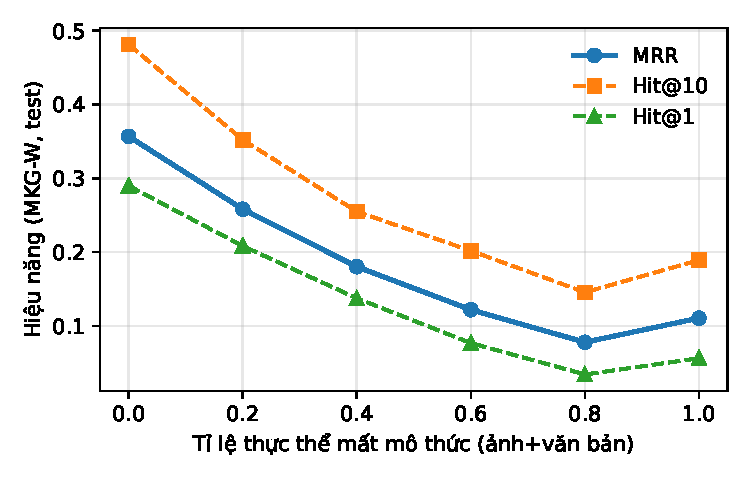
\includegraphics[width=0.92\columnwidth]{figures/fig3_missing.pdf}
\caption{Độ bền của AdaMF khi thiếu mô thức (MKG-W, checkpoint $\mu=0$): hiệu năng theo
tỉ lệ thực thể bị bỏ ảnh$+$văn bản. $p=0$ tái hiện đúng đường cơ sở (MRR $0{,}3568$).}
\label{fig:missing}
\end{figure}

Đường cong này nói hai điều. Thứ nhất, hiệu năng tụt đơn điệu và mạnh khi $p$ tăng từ
$0$ đến $0{,}8$ (MRR $0{,}3568 \to 0{,}0779$), cho thấy mô hình phụ thuộc thực vào mô
thức bổ trợ dù attention gán cho ảnh trọng số rất nhỏ; ảnh không vô dụng mà đóng vai
trò khi riêng cấu trúc chưa đủ. Thứ hai, và bất ngờ hơn, tại $p=1{,}0$ khi mọi thực
thể đều thiếu, MRR lại hồi lên $0{,}1107$, cao hơn mức $0{,}0779$ ở $p=0{,}8$. Lý do
là khi tất cả cùng mất mô thức, không gian biểu diễn trở lại nhất quán ở dạng thuần
cấu trúc, trong khi thiếu một phần tạo ra hỗn hợp không đồng nhất khó khớp hơn. Đây là
một quan sát từ \emph{một} seed và sáu điểm đo (chưa lặp lại nên không kèm thanh sai số),
nên chỉ nên xem là \emph{gợi ý}: chính tính không đồng nhất của dữ liệu thiếu có thể gây
hại hơn cả lượng thiếu, một góc nhìn mà biểu đồ gốc của bài báo không nêu.

\subsection{Bảy điểm không nhất quán bài báo $\leftrightarrow$ mã nguồn}
Tổng hợp từ đọc mã từng dòng và kiểm chứng số:
\begin{enumerate}
  \item Script chính thức \texttt{mu=0} $\Rightarrow$ chạy nguyên bản không ra
  AdaMF-MAT; $\lambda$ thắng không công bố. \emph{(nghiêm trọng)}
  \item Eq.~4 nói trọng số riêng từng mô thức; mã dùng \emph{một} vector chung.
  \item \texttt{dim}: bài báo "200", script DB15K dùng 250.
  \item \texttt{lr=2e-5} nằm ngoài lưới bài báo khai.
  \item Bảng đặc trưng ảnh/văn bản là \emph{khả huấn luyện} (\texttt{requires\_grad
  =True}); riêng bảng ảnh DB15K chiếm 52,6M/71,4M tham số, không phải "$\sim$10M".
  \item Thí nghiệm modality-missing (Figure~3, RQ2) \emph{không có} trong mã phát
  hành: \texttt{-missing\_rate}, \texttt{-visual} được khai trong \texttt{args.py}
  nhưng không nơi nào đọc. Muốn tái lập phải tự viết phần bỏ mô thức. \emph{(nghiêm trọng)}
  \item Table~1 ghi DB15K valid/test là 9902/9904, file thật đảo ngược 9904/9902, bằng chứng bài báo và artifact không được đối soát.
\end{enumerate}
Các phần khớp hoàn toàn: các phương trình RotatE, tập ba bộ ba giả, $K=128$,
$\beta=2$, $\gamma=12$, batch 1024, đánh giá filtered.

Tóm lại phần A, đóng góp thứ hai là MAT không tái lập được từ artifact công bố nếu
không tự dò lại $\lambda$, và hai phương trình lõi (Eq.~4, Eq.~8) mô tả sai chính mã
của tác giả. Cái model thực sự học được là \emph{một} vector attention
dùng chung, không phải trọng số riêng từng mô thức như bài viết.

%##############################################################################
\section*{PHẦN B: MKG-FENN}
%##############################################################################

%==============================================================================
\section{Bài toán dự đoán sự kiện tương tác thuốc}
%==============================================================================

Tương tác thuốc--thuốc (DDI) xảy ra khi dùng đồng thời hai thuốc làm thay đổi
hiệu quả hoặc gây tác dụng phụ. MKG-FENN~\cite{mkgfenn} giải bài toán
\emph{phân loại đa lớp}: cho một cặp thuốc $(A, B)$, dự đoán \emph{loại sự kiện}
tương tác trong 65 loại (\texttt{event\_num=65}), ví dụ "nguy cơ hoặc mức độ tác
dụng phụ tăng lên". Dữ liệu nền gồm 572 thuốc (\texttt{n\_drug=572}) từ DrugBank,
cùng dòng dữ liệu với DDIMDL~\cite{ddimdl}.

Cũng nên hình dung qua một ví dụ. Cho cặp thuốc \texttt{(Abemaciclib, Amiodarone)},
mỗi thuốc được tra đặc trưng từ bốn đồ thị tri thức (thực thể hóa học, cấu trúc con,
DDI, thuộc tính phân tử) qua bốn nhánh KGNN, ghép thành tám vector rồi đưa qua MLP.
Đầu ra là một trong 65 lớp sự kiện, ở đây là "nguy cơ hoặc mức độ tác dụng phụ tăng
lên", đúng với nhãn trong \texttt{event.db} (dòng \texttt{Abemaciclib//Amiodarone//The
risk or severity of adverse effects increase}).

Điểm mấu chốt của bài báo: các phương pháp trước xét quan hệ/cơ chế DDI \emph{rời
rạc} (non-end-to-end), nên trích xuất và hợp nhất đặc trưng chưa tối ưu. MKG-FENN
xây một đồ thị tri thức đa mô thức từ bốn nguồn quan hệ và học hợp nhất
\emph{đầu-cuối} bằng một mạng nơ-ron.

%==============================================================================
\section{Kiến trúc MKG-FENN}
%==============================================================================

\subsection{Bốn đồ thị tri thức ("đa mô thức")}
Bốn đồ thị (Bảng~\ref{tab:kg4}), mỗi đồ thị mô tả thuốc theo một góc nhìn quan hệ
khác nhau, định dạng \texttt{head//tail//relation}.

\begin{table}[t]
\caption{Bốn đồ thị tri thức của MKG-FENN (đọc từ mã).}
\label{tab:kg4}
\centering
\footnotesize
\begin{tabular}{clrr p{2.3cm}}
\toprule
KG & File & \#dòng & \#quan hệ & Nội dung \\
\midrule
G1 & dataset1 & 6.541  & 235 & thuốc--thực thể hóa học (target/enzyme/\dots) \\
G2 & dataset2 & 70.350 & 1   & thuốc--cấu trúc con (chỉ "include") \\
G3 & dataset3 & 37.264 & 65  & thuốc--thuốc (DDI chính) \\
G4 & dataset4 & 11.440 & 13  & thuốc--thuộc tính phân tử (MolWt, MolLogP\dots) \\
\bottomrule
\end{tabular}
\end{table}

Nhãn sự kiện lấy từ \texttt{event.db} (SQLite), nhãn $=$ cơ chế $+$ hành động, sắp
theo tần suất giảm dần thành 65 lớp.

\subsection{Bốn nhánh GNN kiểu KGNN}
Trái với cái tên "GNN" gợi ý message-passing sâu, mã thực thi là kiểu
\emph{lấy mẫu láng giềng $+$ tổng hợp bằng attention} (giống KGNN~\cite{kgnn}).
Với mỗi đồ thị $G_i$ và mỗi thuốc:
\begin{enumerate}
  \item \textbf{Lấy mẫu.} Chọn ngẫu nhiên $K$ láng giềng ($K=6$ mặc định) từ $G_i$
  (\texttt{np.random.choice}, có lặp nếu thiếu), thu tail và quan hệ.
  \item \textbf{Tính trọng số láng giềng.} Với embedding thuốc, quan hệ, thực thể
  (số chiều $d=128$):
  \begin{align}
    \mathbf{d}_{\text{rel}} &= \mathbf{e}_{\text{drug}} \odot \mathbf{e}_{\text{rel}},\\
    \mathbf{s} &= \mathrm{ReLU}(\mathbf{d}_{\text{rel}} W_1 + b_1) W_2 + b_2,\\
    \boldsymbol{\alpha} &= \mathrm{softmax}\!\big(\textstyle\sum \mathbf{s}\big),\\
    \mathbf{e}_{\text{agg}} &= \boldsymbol{\alpha} \cdot \mathbf{e}_{\text{ent}}.
  \end{align}
  \item \textbf{Đặc trưng thuốc theo KG.} Ghép
  $[\mathbf{e}_{\text{agg}}; \mathbf{e}_{\text{drug}}]$ rồi qua Linear
  ($2d\!\to\! d$)$+$ReLU$+$BatchNorm, thu $\mathbf{f}_i$.
\end{enumerate}

\textbf{Bẫy chi phí.} Ma trận $W_1, W_2$ có kích thước $572\times d\times d$,
\emph{riêng cho từng thuốc}. Mỗi nhánh vì thế cần $\approx 572\times128\times128\times2
\approx 18{,}7$ triệu tham số, bốn nhánh cộng lại cỡ $75$ triệu chỉ cho phần KGNN. Đây
là một chi phí tham số đáng kể mà cách mô tả kiến trúc trong bài báo không làm nổi bật,
người đọc khó hình dung nếu chỉ nhìn sơ đồ.

\subsection{Tầng hợp nhất (FusionLayer)}
Với mỗi cặp $(A, B)$, ghép \emph{tám} vector đặc trưng, $\{\mathbf{f}_1,\dots,
\mathbf{f}_4\}$ của $A$ và của $B$, thành $8d = 1024$ chiều, rồi qua MLP
$1024 \to 512 \to 256 \to 65$ (ReLU$+$BN$+$Dropout 0,3), xuất 65 lớp
(Hình~\ref{fig:fenn}). Khi huấn luyện, mỗi cặp được nhân đôi thành $(A,B)$ và
$(B,A)$ để đối xứng hóa.

\begin{figure}[t]
\centering
\begin{tikzpicture}[font=\scriptsize,
  g/.style={draw,rounded corners,fill=blue!8,minimum width=9mm,minimum height=5mm},
  >=Latex,node distance=2mm]
  \node[g] (g1) {$G_1$}; \node[g,below=of g1] (g2) {$G_2$};
  \node[g,below=of g2] (g3) {$G_3$}; \node[g,below=of g3] (g4) {$G_4$};
  \node[draw,rounded corners,fill=green!8,right=8mm of g2,minimum height=16mm,align=center] (fus) {Fusion\\MLP};
  \node[draw,rounded corners,right=6mm of fus] (out) {65 lớp};
  \foreach \i in {1,2,3,4} \draw[->] (g\i) -- (fus);
  \draw[->] (fus) -- (out);
  \node[align=center,below=1mm of g4,font=\tiny] {8 vector = 4 KG $\times$ 2 thuốc};
\end{tikzpicture}
\caption{MKG-FENN: bốn nhánh KGNN sinh đặc trưng thuốc theo từng đồ thị; tầng
hợp nhất ghép tám vector của cặp thuốc rồi phân loại 65 lớp sự kiện.}
\label{fig:fenn}
\end{figure}

%==============================================================================
\section{Đánh giá và nhận xét}
%==============================================================================

\subsection{Ba kịch bản đánh giá}
Mã cung cấp ba tác vụ với độ khó tăng dần:
\begin{itemize}
  \item \textbf{Task 1}: chia ngẫu nhiên, StratifiedKFold 5-fold trên các cặp
  DDI. Dễ nhất: cả hai thuốc đều xuất hiện khi huấn luyện.
  \item \textbf{Task 2}: cold-start theo thuốc (chia theo drug id), kịch bản
  \emph{một} thuốc trong cặp là mới (chưa xuất hiện khi huấn luyện). Khó hơn Task~1.
  \item \textbf{Task 3}: cold-start khó nhất, \emph{cả hai} thuốc trong cặp đều mới.
\end{itemize}
Chỉ số: ACC, AUPR, AUC, F1 (micro/macro), Precision, Recall, bộ 11 chỉ số toàn
cục theo file supplementary.

\subsection{Kết quả chính (theo bài báo)}
Trên kịch bản thuốc đã biết (Task~1, DrugBank v5.1.7, 572 thuốc, 65 sự kiện), bài báo
báo cáo MKG-FENN vượt mọi mô hình so sánh ở toàn bộ 6 chỉ số (Bảng~\ref{tab:fenn-res}, số trích
trực tiếp từ Table~2 của bài báo); tổng thắng $64/66$ so sánh chỉ số $\times$ mô hình
(2 hòa, 0 thua), F-rank cao nhất $11{,}83$.

\begin{table}[t]
\caption{Kết quả Task~1 (số bài báo, trích Table~2 của~\cite{mkgfenn}): MKG-FENN so với các mô hình mạnh.}
\label{tab:fenn-res}
\centering
\footnotesize
\setlength{\tabcolsep}{4pt}
\begin{tabular}{lrrrrrr}
\toprule
Mô hình & ACC & AUPR & AUC & F1 & Pre & Rec \\
\midrule
\textbf{MKG-FENN} & \textbf{0,9409} & \textbf{0,9786} & \textbf{0,9989} & \textbf{0,8958} & \textbf{0,9132} & \textbf{0,8876} \\
MDDI-SCL     & 0,9378 & 0,9782 & 0,9983 & 0,8755 & 0,8804 & 0,8767 \\
MDF-SA-DDI   & 0,9301 & 0,9737 & 0,9989 & 0,8878 & 0,9085 & 0,8760 \\
MDNN         & 0,9175 & 0,9668 & 0,9984 & 0,8301 & 0,8622 & 0,8202 \\
DDIMDL       & 0,8852 & 0,9208 & 0,9976 & 0,7585 & 0,8471 & 0,7182 \\
\bottomrule
\end{tabular}
\end{table}

Một điều lộ rõ qua ba kịch bản là cold-start rất khó. Cùng một mô hình, ACC tụt mạnh
theo độ khó: $0{,}9409$ ở Task~1 (cả hai thuốc đã thấy), xuống $0{,}6805$ ở Task~2
(một thuốc mới), rồi chỉ còn $0{,}4552$ ở Task~3 (cả hai đều mới). Khoảng cách đó cho
thấy phần lớn thành công nằm ở kịch bản dễ, còn dự đoán cho thuốc hoàn toàn mới vẫn là
bài toán mở.

Ba yếu tố quan trọng nhất (phân tích độ nhạy): số láng giềng lấy mẫu tốt nhất $=6$, trọng
số mất mát phân loại (CLW) tốt nhất $=10^{-8}$, số chiều embedding $=128$. Bài dùng $120$
epoch, lr $=0{,}01$, batch $1024$: các giá trị này khớp mã (dù nằm ngoài tập \texttt{choices}
khai trong argparse, nên đây là lỗi khai báo chứ không phải lệch paper$\leftrightarrow$mã).

\subsection{Nhóm tái lập (GPU T4, 3 seed)}
\noindent Báo cáo W\&B của phần này: \url{https://wandb.ai/K35/gml-adamf-mat/reports/VmlldzoxODE3OTk3Nw==}.
Mã nguồn tái lập: \url{https://github.com/lqhung93/graphML-midterm-project}.

Nhóm GPU-hóa mã (thêm \texttt{.to(device)}, mã gốc chỉ chạy CPU) và chạy lại Task~1 (120 epoch,
5-fold) với \textbf{3 seed} (0, 1, 2), mỗi lần $\sim$1 giờ. Trung bình $\pm$ độ lệch chuẩn
\textbf{khớp bài báo ở mọi chỉ số, số bài báo nằm trong khoảng $\pm$std} (Bảng~\ref{tab:fenn-repro})
$\Rightarrow$ MKG-FENN \emph{tái lập được}. Đây là tương phản rõ với
Phần~A, nơi đóng góp MAT của AdaMF-MAT \emph{không} tái lập được: cùng một thái độ kiểm chứng
nghiêm túc cho hai kết luận trái ngược, tùy công trình.

\begin{table}[t]
\caption{MKG-FENN Task~1: nhóm tái lập (3 seed, trung bình $\pm$ độ lệch chuẩn) vs bài báo.}
\label{tab:fenn-repro}
\centering\footnotesize
\begin{tabular}{lrr}
\toprule
Chỉ số & Nhóm (3 seed) & Bài báo \\
\midrule
ACC & $0{,}9403 \pm 0{,}0012$ & 0,9409 \\
AUPR (micro) & $0{,}9783 \pm 0{,}0007$ & 0,9786 \\
AUC (micro) & $0{,}9989 \pm 0{,}0001$ & 0,9989 \\
F1 (macro) & $0{,}8932 \pm 0{,}0041$ & 0,8958 \\
Precision (macro) & $0{,}9202 \pm 0{,}0090$ & 0,9132 \\
Recall (macro) & $0{,}8813 \pm 0{,}0055$ & 0,8876 \\
\bottomrule
\end{tabular}
\end{table}

Nhóm dùng một tiêu chí tái lập thực dụng xuyên suốt báo cáo: xem là \emph{nhất quán với
bài báo} khi con số công bố nằm trong một độ lệch chuẩn mẫu của nhóm qua ba lần chạy độc
lập. Đây là kiểm tra khoảng tin cậy, không phải kiểm định giả thuyết hình thức, nên phát
biểu đúng là "không phân biệt được với số công bố ở mức nhiễu ba seed", chứ không khẳng
định bằng chứng mạnh hơn thế. Theo tiêu chí này, số bài báo nằm trong khoảng ở cả 6 chỉ
số. Link W\&B (3 seed): \url{https://wandb.ai/K35/gml-adamf-mat/runs/bblj2qcv},
\url{https://wandb.ai/K35/gml-adamf-mat/runs/jfcaxbp1},
\url{https://wandb.ai/K35/gml-adamf-mat/runs/t4yt0kks}.

\subsection{Nhóm tái lập cold-start (Task 2 và Task 3)}
\noindent Báo cáo W\&B của phần này: \url{https://wandb.ai/K35/gml-adamf-mat/reports/VmlldzoxODE3OTk3OA==}.

Nhóm chạy lại luôn kịch bản khó Task~2 (cold-start, một thuốc mới) với \textbf{3 lần}
độc lập (GPU T4, 120 epoch, mỗi lần $\sim$1 giờ). ACC trung bình $0{,}6772 \pm 0{,}0039$,
\textbf{số bài báo $0{,}6805$ nằm trong khoảng $\pm$ độ lệch chuẩn} (Bảng~\ref{tab:fenn-t2})
$\Rightarrow$ tái lập được cả ở kịch bản cold-start, không chỉ Task~1 dễ. Lưu ý mã Task~2
chỉ tính AUPR/AUC theo micro và F1/Precision/Recall theo macro (các ô còn lại gán cứng
bằng $0$, nhóm không ghi các ô này lên W\&B), nên AUPR mà bài báo báo ở Table~3/4 thực
chất là AUPR micro; cách
trung bình macro trên nhiều lớp sự kiện hiếm khiến F1/Precision/Recall thấp hơn hẳn Task~1,
phản ánh đúng độ khó của dự đoán cho thuốc chưa từng thấy.

\begin{table}[t]
\caption{MKG-FENN Task~2 (cold-start, một thuốc mới): nhóm tái lập (3 lần, trung bình $\pm$ độ lệch chuẩn).}
\label{tab:fenn-t2}
\centering\footnotesize
\begin{tabular}{lrr}
\toprule
Chỉ số & Nhóm (3 lần) & Bài báo \\
\midrule
ACC & $0{,}6772 \pm 0{,}0039$ & 0,6805 \\
AUPR (micro) & $0{,}7010 \pm 0{,}0015$ & -- \\
AUC (micro) & $0{,}9663 \pm 0{,}0008$ & -- \\
F1 (macro) & $0{,}5294 \pm 0{,}0045$ & -- \\
Precision (macro) & $0{,}5862 \pm 0{,}0075$ & -- \\
Recall (macro) & $0{,}5045 \pm 0{,}0071$ & -- \\
\bottomrule
\end{tabular}
\end{table}

Link W\&B (3 lần): \url{https://wandb.ai/K35/gml-adamf-mat/runs/jytx7d9z},
\url{https://wandb.ai/K35/gml-adamf-mat/runs/7dqjvbo0},
\url{https://wandb.ai/K35/gml-adamf-mat/runs/zh74tvnv}.

Nhóm chạy tiếp \textbf{Task~3} (cold-start, \emph{cả hai} thuốc mới: khó nhất), cũng 3 lần
(Bảng~\ref{tab:fenn-t3}). ACC trung bình $0{,}4598 \pm 0{,}0175$, \textbf{số bài báo $0{,}4552$
nằm trong $\pm$ độ lệch chuẩn} $\Rightarrow$ tái lập được ở cả ba kịch bản. Chỉ số F1/Precision/
Recall (macro) tụt sâu ($\sim$0,21--0,26) đúng như kỳ vọng khi mọi cặp thuốc đều chưa từng thấy.
Nhóm phải tự GPU-hóa mã Task~3 (giống Task~2) vì bản gốc chỉ chạy CPU.

\begin{table}[t]
\caption{MKG-FENN Task~3 (cold-start, cả hai thuốc mới): nhóm tái lập (3 lần, trung bình $\pm$ độ lệch chuẩn).}
\label{tab:fenn-t3}
\centering\footnotesize
\begin{tabular}{lrr}
\toprule
Chỉ số & Nhóm (3 lần) & Bài báo \\
\midrule
ACC & $0{,}4598 \pm 0{,}0175$ & 0,4552 \\
AUPR (micro) & $0{,}4140 \pm 0{,}0165$ & -- \\
AUC (micro) & $0{,}9153 \pm 0{,}0014$ & -- \\
F1 (macro) & $0{,}2162 \pm 0{,}0076$ & -- \\
Precision (macro) & $0{,}2618 \pm 0{,}0092$ & -- \\
Recall (macro) & $0{,}2097 \pm 0{,}0107$ & -- \\
\bottomrule
\end{tabular}
\end{table}

Link W\&B (3 lần): \url{https://wandb.ai/K35/gml-adamf-mat/runs/h8npelov},
\url{https://wandb.ai/K35/gml-adamf-mat/runs/p4n9in0o},
\url{https://wandb.ai/K35/gml-adamf-mat/runs/19sj3za2}. Cả ba kịch bản cold-start đều tái lập
được (số bài báo nằm trong 1 độ lệch chuẩn), nghĩa là các con số chính của MKG-FENN
\emph{đáng tin}, tương phản với MAT của AdaMF-MAT (Phần~A). Đây là nhận định về
\emph{tính tái lập}, không phải về giá trị kiến trúc: ngược lại, ablation ở dưới cho thấy
tiền đề "cần đủ bốn đồ thị" của chính bài không tái lập được ở Task~1.

\subsection{Ablation KG: bỏ một đồ thị không làm giảm ACC Task 1}
\noindent Báo cáo W\&B của phần này: \url{https://wandb.ai/K35/gml-adamf-mat/reports/VmlldzoxODE3OTk3OQ==}.

Nhóm bỏ từng đồ thị khỏi FusionLayer (Task~1, seed 0, Bảng~\ref{tab:fenn-abl}) bằng cách
gán embedding của nhánh đó bằng $0$. Kích thước đầu vào MLP giữ nguyên, nhưng các trọng số
nhận đầu vào $0$ không còn tác dụng, nên tương đương bỏ hẳn nhánh. \textbf{Bỏ bất kỳ KG nào,
kể cả đồ thị DDI (G3), đều không làm giảm ACC}: cả bốn cấu hình (0,9398 đến 0,9411) nằm
trong dải của ba seed mô hình đầy đủ (0,9389 đến 0,9410). Vì mỗi cấu hình chỉ một seed,
nhóm không kết luận cấu hình nào tốt hơn full; điều đọc được là \emph{không thấy} mức giảm
vượt nhiễu giữa seed. Điều này lệch với Table~5 của bài báo: ở đó cả bốn tổ hợp ba đồ thị
chỉ đạt 0,9344 đến 0,9355, thấp hơn full $\sim$0,6 điểm, tức gấp khoảng năm lần độ lệch
chuẩn giữa seed của nhóm ($0{,}0012$). Bài báo không nói cách bỏ kênh, nên khác biệt có thể
một phần do cách cài đặt. \emph{Phạm vi:} nhóm chỉ chạy bốn cấu hình bỏ một đồ thị trong
15 tổ hợp của Table~5, chỉ trên Task~1; cold-start (Task~2/3) có thể khác.

\begin{table}[t]
\caption{MKG-FENN KG-ablation (Task~1, seed 0): bỏ 1 đồ thị.}
\label{tab:fenn-abl}
\centering\footnotesize
\begin{tabular}{llrr}
\toprule
Bỏ & Nội dung & ACC & F1 (macro) \\
\midrule
(full) & 4 đồ thị & 0,9389 & 0,8944 \\
G1 & hóa học & 0,9409 & 0,8943 \\
G2 & cấu trúc con & 0,9399 & 0,8956 \\
G3 & DDI & 0,9411 & 0,9000 \\
G4 & phân tử & 0,9398 & 0,8982 \\
\bottomrule
\end{tabular}
\end{table}

\subsection{Phân tích độ nhạy siêu tham số (Task 1, seed 0)}
Nhóm quét lại hai siêu tham số bài báo nhấn mạnh: số láng giềng lấy mẫu
(\texttt{neighbor\_sample\_size}) và số chiều embedding (\texttt{embedding\_num}),
mỗi giá trị một lần (seed 0) trên GPU T4 (Bảng~\ref{tab:fenn-sens}). Với
\texttt{neighbor\_sample\_size}, ACC dao động 0,9389 đến 0,9410, đúng bằng dải của ba seed
mô hình gốc, nên nhóm không phân biệt được các giá trị với nhau và cũng không xác nhận được
"số láng giềng $=6$ tốt nhất" như bài báo. Với \texttt{embedding\_num}, $32$ chiều kém rõ
($-1{,}4$ điểm, khoảng mười hai lần độ lệch chuẩn giữa seed), nên ảnh hưởng của dung lượng mô hình ở
đầu thấp là thật; còn chênh giữa $64$, $128$ và $256$ (tối đa $+0{,}36$ điểm) cần thêm seed
mới kết luận được, trong khi $256$ tốn gấp $2{,}5$ lần thời gian. Nhóm chưa quét tham số
thứ ba bài báo nêu là trọng số loss phân loại (CLW).

\begin{table}[t]
\caption{MKG-FENN độ nhạy siêu tham số (Task~1, seed 0). ACC $=$ micro.}
\label{tab:fenn-sens}
\centering\footnotesize
\begin{tabular}{lrrr}
\toprule
Siêu tham số & Giá trị & ACC & F1 (macro) \\
\midrule
\texttt{neighbor\_sample\_size} & 4 & 0,9409 & 0,8939 \\
 & 6 (gốc) & 0,9389 & 0,8944 \\
 & 10 & 0,9410 & 0,8979 \\
 & 16 & 0,9390 & 0,8940 \\
\midrule
\texttt{embedding\_num} & 32 & 0,9246 & 0,8466 \\
 & 64 & 0,9384 & 0,8867 \\
 & 128 (gốc) & 0,9389 & 0,8944 \\
 & 256 & 0,9425 & 0,8965 \\
\bottomrule
\end{tabular}
\end{table}

Sáu run này nằm cùng báo cáo W\&B với ablation đồ thị: \url{https://wandb.ai/K35/gml-adamf-mat/reports/VmlldzoxODE3OTk3OQ==}.

\subsection{Bẫy tái lập của MKG-FENN}
Ngoài số tái lập trên, đọc mã còn lộ vài điểm cần lưu
nếu ai muốn tái lập:
\begin{enumerate}
  \item Repo chỉ có \texttt{event.rar}, mã lại cần \texttt{event.db}; phải giải
  nén trước, nếu không \texttt{sqlite3.connect} sẽ lỗi.
  \item GNN3 hardcode \texttt{num\_embeddings=67} cho bảng quan hệ trong khi
  dataset3 chỉ có 65 quan hệ (đệm $+2$), cần kiểm off-by-two là cố ý hay lỗi.
  \item Mặc định \texttt{lr=1e-2} và \texttt{epoches=120} nằm \emph{ngoài} tập
  \texttt{choices} khai trong argparse, giá trị thật khác lưới liệt kê.
  \item Lấy mẫu láng giềng ngẫu nhiên \emph{mỗi lần forward} $\Rightarrow$ kết quả
  có phương sai giữa các lần chạy dù đã cố định seed. Nên báo cáo trung bình nhiều
  lần thay vì một con số.
\end{enumerate}

\subsection{So sánh hai công trình}
Bảng~\ref{tab:compare} đặt cạnh hai cách "hợp nhất trên đồ thị".

\begin{table}[t]
\caption{Đối chiếu hai công trình.}
\label{tab:compare}
\centering
\footnotesize
\begin{tabular}{p{2.1cm} p{2.4cm} p{2.4cm}}
\toprule
& AdaMF-MAT & MKG-FENN \\
\midrule
Tác vụ & hoàn thiện KG (link prediction) & phân loại sự kiện DDI (65 lớp) \\
Hợp nhất & các \emph{mô thức} (cấu trúc/ảnh/văn bản) & các \emph{loại quan hệ} (4 đồ thị) \\
Xương sống & RotatE $+$ đối kháng & KGNN 4 nhánh $+$ MLP \\
Đầu-cuối & có & có \\
Nhóm chạy lại & có (MKG-W, MKG-Y, DB15K) & có (Task 1/2/3, ablation, quét siêu tham số) \\
\bottomrule
\end{tabular}
\end{table}

%==============================================================================
\section{Kết luận}
%==============================================================================

Hai công trình cùng theo đuổi hợp nhất có học trên đồ thị tri thức đa mô thức
nhưng cho hai bài học trái ngược về tính tái lập.

Với AdaMF-MAT, nhóm quét trọn lưới hệ số MAT trên \emph{ba} tập dữ liệu (MKG-W có
thêm ba seed, MKG-Y, và DB15K chạy đủ 1000 epoch bằng cơ chế resume tự thêm). Trên
cả ba, đóng góp cốt lõi thứ hai là MAT không tái lập được mức đã công bố: ở MKG-W
chỉ $+0{,}06 \pm 0{,}07$ MRR so với $+1{,}58$, và ngay tại DB15K nơi bài báo khai MAT
mạnh nhất ($+2{,}63$) thì cấu hình đã thử lại \emph{giảm} $0{,}41$, trong khi đường cơ
sở không MAT của nhóm còn vượt chính hàng AdaMF-MAT của bài báo. Phần hợp nhất thích
nghi hoá ra học cách loại bỏ mô thức ảnh, và thí nghiệm thiếu mô thức mà nhóm tự viết
(tái lập Figure~3) còn gợi ý rằng tính không đồng nhất của dữ liệu thiếu gây hại hơn
cả lượng thiếu.

Với MKG-FENN, cả ba kịch bản (biết thuốc và hai mức cold-start) đều tái lập trong một
độ lệch chuẩn, nên các con số chính đáng tin; nhưng ablation của nhóm không tái lập
được mức giảm khi bỏ một đồ thị mà Table~5 báo cáo, và kiến trúc tuy gọn về ý tưởng lại nặng
về tham số ($W_1,W_2$ riêng từng thuốc). Cả hai trường hợp củng cố nguyên tắc làm việc
của nhóm: không tin một phát biểu trong bài báo cho đến khi chỉ được dòng mã thực thi nó.

%==============================================================================
\appendices
\section{Ánh xạ thực nghiệm $\to$ liên kết Weights \& Biases}
\label{app:wandb}
%==============================================================================

Toàn bộ \textbf{40 run} đều ở chế độ xem công khai trong project
\url{https://wandb.ai/K35/gml-adamf-mat}. Danh sách đầy đủ liên kết từng thí nghiệm:

\par\smallskip\noindent\textbf{AdaMF-MAT, MKG-W (nhiều seed, ablation mô thức, trọng số attention):}
\begin{itemize}\itemsep0pt\parskip0pt
  \item $\mu{=}0$ seed 42: \url{https://wandb.ai/K35/gml-adamf-mat/runs/p0o2czqu}
  \item $\mu{=}0$ seed 1: \url{https://wandb.ai/K35/gml-adamf-mat/runs/xqu9bfhm}
  \item $\mu{=}0$ seed 2: \url{https://wandb.ai/K35/gml-adamf-mat/runs/5lh1mfbz}
  \item $\mu{=}0{,}001$ seed 42: \url{https://wandb.ai/K35/gml-adamf-mat/runs/lkvk7l7q}
  \item $\mu{=}0{,}001$ seed 1: \url{https://wandb.ai/K35/gml-adamf-mat/runs/jif9r05n}
  \item $\mu{=}0{,}001$ seed 2: \url{https://wandb.ai/K35/gml-adamf-mat/runs/vq1hsz68}
  \item $\mu{=}0{,}01$ seed 42: \url{https://wandb.ai/K35/gml-adamf-mat/runs/xgvzh5qi}
  \item $\mu{=}0{,}1$ seed 42: \url{https://wandb.ai/K35/gml-adamf-mat/runs/om09b4oc}
  \item ablation bỏ cấu trúc: \url{https://wandb.ai/K35/gml-adamf-mat/runs/hmefe899}
  \item ablation bỏ ảnh: \url{https://wandb.ai/K35/gml-adamf-mat/runs/zz3c5tlx}
  \item ablation bỏ văn bản: \url{https://wandb.ai/K35/gml-adamf-mat/runs/nfqjzksh}
  \item trọng số mô thức (Figure 5) seed 42: \url{https://wandb.ai/K35/gml-adamf-mat/runs/2os78m84}
  \item trọng số mô thức seed 1: \url{https://wandb.ai/K35/gml-adamf-mat/runs/hipyhujk}
  \item trọng số mô thức seed 2: \url{https://wandb.ai/K35/gml-adamf-mat/runs/899aimo9}
  \item thiếu mô thức (Figure 3): \url{https://wandb.ai/K35/gml-adamf-mat/runs/91r5gpjc}
\end{itemize}
\par\smallskip\noindent\textbf{AdaMF-MAT, MKG-Y (lưới $\mu$):}
\begin{itemize}\itemsep0pt\parskip0pt
  \item $\mu{=}0$: \url{https://wandb.ai/K35/gml-adamf-mat/runs/8mh8ill2}
  \item $\mu{=}0{,}001$: \url{https://wandb.ai/K35/gml-adamf-mat/runs/4v6mfwrb}
  \item $\mu{=}0{,}01$: \url{https://wandb.ai/K35/gml-adamf-mat/runs/h3wtr29y}
  \item $\mu{=}0{,}1$: \url{https://wandb.ai/K35/gml-adamf-mat/runs/ws0tp5zq}
\end{itemize}
\par\smallskip\noindent\textbf{AdaMF-MAT, DB15K (1000 epoch):}
\begin{itemize}\itemsep0pt\parskip0pt
  \item $\mu{=}0$ (không MAT): \url{https://wandb.ai/K35/gml-adamf-mat/runs/cih2im9c}
  \item $\mu{=}0{,}01$ (MAT): \url{https://wandb.ai/K35/gml-adamf-mat/runs/up5yivan}
\end{itemize}
\par\smallskip\noindent\textbf{MKG-FENN, Task 1 (3 seed, ablation đồ thị, độ nhạy siêu tham số):}
\begin{itemize}\itemsep0pt\parskip0pt
  \item seed 0: \url{https://wandb.ai/K35/gml-adamf-mat/runs/bblj2qcv}
  \item seed 1: \url{https://wandb.ai/K35/gml-adamf-mat/runs/jfcaxbp1}
  \item seed 2: \url{https://wandb.ai/K35/gml-adamf-mat/runs/t4yt0kks}
  \item bỏ G1: \url{https://wandb.ai/K35/gml-adamf-mat/runs/mo4jlgsr}
  \item bỏ G2: \url{https://wandb.ai/K35/gml-adamf-mat/runs/jfkkfhek}
  \item bỏ G3: \url{https://wandb.ai/K35/gml-adamf-mat/runs/gwlkl9ah}
  \item bỏ G4: \url{https://wandb.ai/K35/gml-adamf-mat/runs/3oooqjjx}
  \item ns$=$4: \url{https://wandb.ai/K35/gml-adamf-mat/runs/zod0impb}
  \item ns$=$10: \url{https://wandb.ai/K35/gml-adamf-mat/runs/a7nq24bw}
  \item ns$=$16: \url{https://wandb.ai/K35/gml-adamf-mat/runs/02mq1hfe}
  \item emb$=$32: \url{https://wandb.ai/K35/gml-adamf-mat/runs/zs388s5c}
  \item emb$=$64: \url{https://wandb.ai/K35/gml-adamf-mat/runs/z1l20qol}
  \item emb$=$256: \url{https://wandb.ai/K35/gml-adamf-mat/runs/odrck7dp}
\end{itemize}
\par\smallskip\noindent\textbf{MKG-FENN, cold-start (Task 2 và Task 3):}
\begin{itemize}\itemsep0pt\parskip0pt
  \item Task 2 lần 1: \url{https://wandb.ai/K35/gml-adamf-mat/runs/jytx7d9z}
  \item Task 2 lần 2: \url{https://wandb.ai/K35/gml-adamf-mat/runs/7dqjvbo0}
  \item Task 2 lần 3: \url{https://wandb.ai/K35/gml-adamf-mat/runs/zh74tvnv}
  \item Task 3 lần 1: \url{https://wandb.ai/K35/gml-adamf-mat/runs/h8npelov}
  \item Task 3 lần 2: \url{https://wandb.ai/K35/gml-adamf-mat/runs/p4n9in0o}
  \item Task 3 lần 3: \url{https://wandb.ai/K35/gml-adamf-mat/runs/19sj3za2}
\end{itemize}

\begin{thebibliography}{9}
\bibitem{adamfmat}
Y. Zhang, Z. Chen, L. Liang, H. Chen, and W. Zhang,
``Unleashing the Power of Imbalanced Modality Information for Multi-modal
Knowledge Graph Completion,'' in \emph{Proc. LREC-COLING}, 2024.
arXiv:2402.15444.

\bibitem{mkgfenn}
D. Wu, W. Sun, Y. He, Z. Chen, and X. Luo,
``MKG-FENN: A Multimodal Knowledge Graph Fused End-to-end Neural Network for
Accurate Drug--Drug Interaction Prediction,'' in \emph{Proc. AAAI}, vol.~38,
no.~9, 2024, pp.~10216--10224. DOI:~10.1609/aaai.v38i9.28887.

\bibitem{rotate}
Z. Sun, Z.-H. Deng, J.-Y. Nie, and J. Tang,
``RotatE: Knowledge Graph Embedding by Relational Rotation in Complex Space,''
in \emph{Proc. ICLR}, 2019.

\bibitem{kgnn}
X. Lin, Z. Quan, Z.-J. Wang, T. Ma, and X. Zeng,
``KGNN: Knowledge Graph Neural Network for Drug--Drug Interaction Prediction,''
in \emph{Proc. IJCAI}, 2020, pp.~2739--2745.

\bibitem{ddimdl}
Y. Deng, X. Xu, Y. Qiu, J. Xia, W. Zhang, and S. Liu,
``A multimodal deep learning framework for predicting drug--drug interaction
events,'' \emph{Bioinformatics}, vol.~36, no.~15, pp.~4316--4322, 2020.

\bibitem{openke}
X. Han et al.,
``OpenKE: An Open Toolkit for Knowledge Embedding,''
in \emph{Proc. EMNLP (System Demonstrations)}, 2018, pp.~139--144.

\bibitem{wandb}
L. Biewald,
``Experiment Tracking with Weights and Biases,'' 2020. [Online].
Available: \url{https://www.wandb.com/}

\end{thebibliography}

\end{document}
